\section{A model of human behavior for \ac{WCA}}\label{sec:model}


In order to accurately emulate the behavior of a human, a model for \ac{WCA} needs to implement two main behaviors.
One, it needs to generate realistic execution times for each step in the task, considering the current and historical impairment of the \ac{WCA} system.
And two, it needs to produce sequences of input samples for each step mimicking what a real human would generate.

\subsection{Generating realistic execution times}

As expressed in \cref{ssec:plos}, for ~\cite{olguinmunoz:impact2021} we collected timing and task performance data for \num{40} participants performing a \num{169}-step task, guided by a \ac{WCA}, as well as personality trait scores for each participant.
For this paper, we use this data to construct a probabilistic model for the generation of realistic execution times.
The data is pre-processed to group execution time values by level of neuroticism, previous \acp{TTF}, and duration of impairment.
The resulting collections of execution times represent the distributions of these values for users with specific levels of neuroticism, interacting with systems at specific states of impairment and recent histories of impairment.
These distributions can then be sampled to produce new, realistic execution times.
In the following, we detail the step-by-step processing of this data and construction of the probabilistic model.

\begin{table}
\centering
\caption[A]{%
    Sample of the execution time data  used for the elaboration of the timing model.
    Rows contain the execution times and \acp{TTF} for each of the \num{169} steps performed by the \num{40} participants in \textcite{olguinmunoz:impact2021}, expressed in seconds, together with a unique identifier for the subject, their associated level of normalized neuroticism, and a sequence number identifying the position of the step in the task.
}\label{tab:data:exectime}
\begin{tabular}{rrrrrr}
    \toprule
    {seq} & {run\_id} & {exec\_time} & {ttf} & {neuroticism}\\
    \midrule
    1 & 134146 & 3.655 & 0.597 & 0.375\\
    2 & 134146 & 4.439 & 0.554 & 0.375\\
    3 & 134146 & 2.943 & 0.562 & 0.375\\
    \( \cdots \) & \( \cdots \) & \( \cdots \) & \( \cdots \) & \( \cdots \) \\
    169 & 134146 & 3.532 & 4.571 & 0.375\\
    1 & 134470 & 3.461 & 0.561 & 0.594\\
    2 & 134470 & 6.678 & 0.572 & 0.594\\
    \( \cdots \) & \( \cdots \) & \( \cdots \) & \( \cdots \) & \( \cdots \) \\
    \( \cdots \) & \( \cdots \) & \( \cdots \) & \( \cdots \) & \( \cdots \) \\
    169 & 137353 & 4.615 & 0.537 & 0.625\\
    \bottomrule
    \end{tabular}
\end{table}

We employ a cleaned and re-parameterized copy of the aforementioned timing data.
The \num{6760} data points are arranged in a table, a sample of which can be seen in \cref{tab:data:exectime}, together with identifiers for the subjects, their neuroticism score, and a sequence number for each step.

We begin by discretizing normalized neuroticism into \emph{low} and \emph{high} ranges, \( [0.0, 0.5) \) and \( [0.5, 1.0) \) respectively. 
We also bin \ac{TTF} into terciles; we will refer to the first, second, and third terciles of \ac{TTF} as \emph{low}, \emph{medium}, and \emph{high impairment}.

The next steps of processing are slightly more complex.
For the data of each subject (which we will refer to as a \emph{run}), we shift the execution times by one sample such that each \ac{TTF} measurement (and therefore, impairment level) is associated with the execution time for the next step.
This comes directly from our discussions in \cref{sec:background} and~\cite{olguinmunoz:impact2021}.
Users notice the impairment of the current step only when they have finished it, and thus system impairment has no effect on the execution time of the current step, but directly affects the next one.

We then assign a label to each sample indicating the class of the most recent transition in impairment level in the run.
In other words, for each recorded step, we look back until we find a step with a different level of impairment and assign a label to the current step according to whether that change was from a higher to a lower level of impairment or vice-versa.
However, if the current step is too far from the latest transition in impairment (by default, more than \num{8} steps), it is instead marked as \emph{no transition}; this label is also used for steps at the beginning of each run which have no previous transition in impairment.
This labeling allows us to capture the behavior described in \cref{item:remain} of \cref{ssec:plos}.

Finally, we assign a number to each sample corresponding to \emph{how long} the current combination of level of impairment and transition has been in effect, in number of steps.
This count resets whenever this combination changes.
This value is subsequently discretized into bins with edges \( [0, 5) \), \( [5, 10) \), and \( [10, \infty) \); we will refer to these discretized levels as \emph{short}, \emph{medium}, and \emph{long duration}, respectively.

The results of this processing on the samples from \cref{tab:data:exectime} can be seen in \cref{tab:data:exectime:processed}.
Three examples of the effect of this discretization and processing on the data are also presented in \cref{fig:timing}.

\begin{table*}
\caption{Sample of the processed execution time data table.}\label{tab:data:exectime:processed}
\begin{tabular}{rrrrcrccrc}
\toprule
{seq} & {run\_id} & {next\_exec\_time} & {ttf} & {impairment} & {neuroticism\_raw} & {neuroticism} & {transition} & {duration\_raw} & {duration} \\
\midrule
1   & 134146 & 3.655 & 0.000 & low & 0.375  & low & NoTransition & 1 & short \\
2   & 134146 & 4.439 & 0.597 & low & 0.375 & low & NoTransition & 2 & short \\
3   & 134146 & 2.943 & 0.554 & low & 0.375 & low & NoTransition & 3 & short \\
\( \cdots \) & \( \cdots \) & \( \cdots \) & \( \cdots \) & \( \cdots \) & \( \cdots \) & \( \cdots \) & \( \cdots \) & \( \cdots \) & \( \cdots \)\\
169 & 134146 & 3.532 & 3.689 & high & 0.375 & low & Lower2Higher & 2 & short \\
1   & 134470 & 3.461 & 0.000 & low & 0.594 & high & NoTransition & 1 & short \\
2   & 134470 & 6.678 & 0.561 & low & 0.594 & high & NoTransition & 2 & short \\
\( \cdots \) & \( \cdots \) & \( \cdots \) & \( \cdots \) & \( \cdots \) & \( \cdots \) & \( \cdots \) & \( \cdots \) & \( \cdots \) & \( \cdots \)\\
\( \cdots \) & \( \cdots \) & \( \cdots \) & \( \cdots \) & \( \cdots \) & \( \cdots \) & \( \cdots \) & \( \cdots \) & \( \cdots \) & \( \cdots \)\\
169 & 137353 & 4.615 & 0.579 & low & 0.625 & high & NoTransition & 2 & short \\
\bottomrule
\end{tabular}
\end{table*}

\begin{figure*}
    \centering
    \begin{subfigure}[t]{\columnwidth}
        \centering
        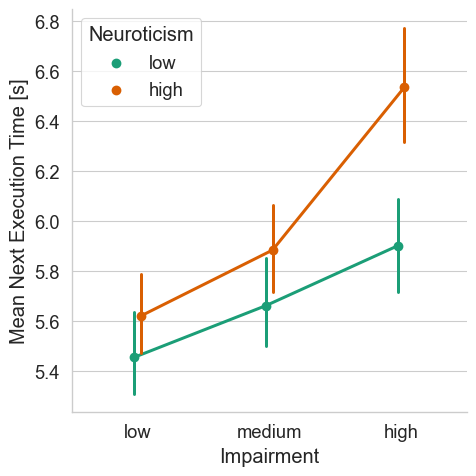
\includegraphics[width=.8\columnwidth]{./model_data/imp_neur_vs_exectime.png}
        \caption{}\label{fig:timing:impneurvsetime}
    \end{subfigure}\\
    \begin{subfigure}[t]{\columnwidth}
        \centering
        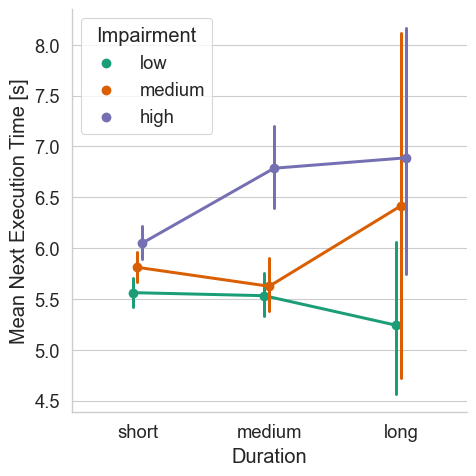
\includegraphics[width=.8\columnwidth]{./model_data/duration_vs_exectime.png}
        \caption{}\label{fig:timing:durvsetime}
    \end{subfigure}%
    \begin{subfigure}[t]{\columnwidth}
        \centering
        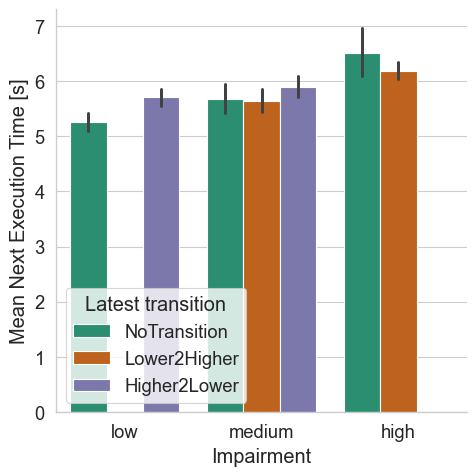
\includegraphics[width=.8\columnwidth]{./model_data/impairment_transition_vs_exectime.png}
        \caption{}\label{fig:timing:imptransvsetime}
    \end{subfigure}
    \caption{%
        Visualizations of the model data after discretization and post-processing.
        \subref{fig:timing:impneurvsetime} illustrates the effect of impairment on execution times, and how neuroticism modulates this behavior;
        \subref{fig:timing:durvsetime} exemplifies how the model captures the speed-up and slow-down behaviors due to impairment and duration described in \textcite{olguinmunoz:impact2021};
        finally, \subref{fig:timing:imptransvsetime} shows the lingering effects of impairment after a transition.
    }\label{fig:timing}
\end{figure*}

\todo[inline]{Diagram of model?}
\todo[inline]{Verification: do we need the model? (Compare to naive)}

\begin{algorithm}
    \caption{Timing model algorithm}
    \KwIn{%
        \begin{itemize}
            \item $T_\text{start}$: start timestamp of the previous step.
            \item $T_\text{success}$: capture timestamp of the succesful sample of the previous step.
            \item $T_\text{end}$: end timestamp of the previous step.
            \item $t_\text{exec}$: execution time (in seconds) of the previous step.
        \end{itemize}%
    }
    \KwOut{$t_\text{exec}'$: execution time for the current step.}

    \Comment{%
        Initial values:\\
        $d \leftarrow 0$\\
        $I_\text{prev} \leftarrow \text{NULL}$
    }
    $t_\text{wait} \leftarrow T_\text{success} - (T_\text{start} + t_\text{exec})$\;
    $t_\text{round-trip} \leftarrow T_\text{end} - T_\text{success}$\;
    $i \leftarrow t_\text{wait} + t_\text{round-trip}$ \Comment*[r]{raw impairment}
    $I \leftarrow \text{BIN}(i)$ \Comment*[r]{bin impairment into\\discrete levels}

    \If{$I_\text{prev} == \text{NULL}$}{%
        $d \leftarrow 1$\;
        $T \leftarrow \text{NO TRANSITION}$\;
    } \ElseIf{$I_\text{prev} < I$}{%
        $d \leftarrow 1$\;
        $T \leftarrow \text{LOWER TO HIGHER} $
    } \ElseIf{$I_\text{prev} > I$}{%
        $d \leftarrow 1$\;
        $T \leftarrow \text{HIGHER TO LOWER} $  
    }

\end{algorithm}


\subsection{Model implementation}

The model is provided as a Python~\num{3.10} library which includes \acp{API} for the generation of realistic execution times and synthetic traces of video frames.

\subsection{Verifying the model}